%!TeX spellcheck = en_US
\documentclass[12pt,a4paper,USenglish]{article}      % Specifies the document class
\usepackage[utf8]{inputenc}
\usepackage[T1]{fontenc,url}
\usepackage{babel,csquotes,newcent,textcomp}
%\usepackage[backend=biber,sortcites]{biblatex}
\usepackage[backend=biber, maxbibnames=99]{biblatex}
\usepackage{graphicx}
%\usepackage{graphics}
%\usepackage{listings}

%\usepackage[options]{duomasterforside}
\usepackage{babel,duomasterforside}

\usepackage{listings}
\usepackage{color}
\usepackage{comment}

\definecolor{dkgreen}{rgb}{0,0.6,0}
\definecolor{gray}{rgb}{0.5,0.5,0.5}
\definecolor{mauve}{rgb}{0.58,0,0.82}

\lstset{frame=tb,
  language=Java,
  aboveskip=3mm,
  belowskip=3mm,
  showstringspaces=false,
  columns=flexible,
  basicstyle={\small\ttfamily},
  numbers=left,
  numberstyle=\tiny\color{gray},
  keywordstyle=\color{blue},
  commentstyle=\color{dkgreen},
  stringstyle=\color{mauve},
  breaklines=true,
  breakatwhitespace=true,
  tabsize=3
}

\addbibresource{mini.bib}

\graphicspath{ {./images/} }

%\addbibresource{References.bib}

\title{Min tittel}  % Declares the document's title.
%\subtitle{Et resultat av to års arbeid}
\author{Svein Gunnar Fagerheim}
%\newcommand{\ip}[2]{(#1, #2)}

\begin{document}             % End of preamble and beginning of text.
%\maketitle                   % Produces the title.

\duoforside[dept={Institutt for informatikk}, program={Informatikk: Programming and System Architecture}, long]

\section{Abstract}
High performance computing is to process data and do calculation on that data at high speed. Traditionally high performance computing uses dynamic random access memory in their computers. 

This thesis will explore an alternative form of memory called persistent memory that will occupy half the DIMM slots in the computer. The persistent memory will be tested for its performance will be compared to traditional memory. The performance will also be tested in competition with traditional memory and its performance will be evaluated.

Persistent memory will also be tested in a more real life setting where persistent memory and traditional memory must cooperate in order to complete their tasks. Its ability to perform independently will also be tested in a more real life example. 


\section{Acknowledgements}
Tekst kommer

\tableofcontents

\section{Introduction}
High performance computing is to process data and do calculation on that data at high speed. The amount of data that is being generated is increasing every year. The data that is being generated in the biggest projects exceeds the capacity of traditional memory. Traditional memory in this context is dynamic random access memory(DRAM).
Traditional way this is solved is to make use of the hard drive which is making the processing and calculation of data significant slower.

A possible solution to this problem could be to use NVDIMM. This is a persistent random-access memory[ref], the difference between DRAM and NVDIMM is that data will not be deleted from NVDIMM when the computer shuts down. 
It has a faster load/store than a hard drive, but is also slower than traditional DRAM. Since NVDIMM is persistent it can also be used as a storage device the same way as traditional hard drives.

\begin{comment}
One way of counter this is to use a new form of storage that is called persistent memory. This is a storage device that is installed in memory slots on the motherboard. It has a faster load/store than a hard drive, but is also slower than traditional DRAM.

This thesis will try to find out how fast the persistent memory really is by doing different types of benchmarks to measure the performance and compare the performance to traditional memory.
The thesis will also explore how the persistent memory performs in experiments that simulates what persistent memory might be used for in the real world. The goal is to come up with a methodology so that other users can quickly set up their processes in a way that make use of persistent memory in the most efficient way possible.
\end{comment}

This thesis will explore several things. First is to explore how fast NVDIMM is compared to DRAM when NVDIMM is working alone. The speed of NVDIMM and DRAM will also be measured when they are working simultaneously, they will be made to work simultaneously using the openMP library.
The thesis will also explore how the persistent memory performs in experiments that simulate what persistent memory might be used for in the real world. The goal is to come up with a set of advice that may help other people who are using NVDIMM in their projects.

The rest of this chapter will describe what persistent memory is and how it will be used in this thesis. There will also a explanation of the challenges and advantages of persistent memory such as cost, durability and persistent memory leak.

\subsection{What is persistent memory}
Persistent memory\cite{Rudoff2} is a non-volatile storage memory\cite{Mahmut} that is byte-addressable and has speed close to that of DRAM. DRAM stands for direct random-access memory, this is a volatile storage system that will lose all its data when the computer is shut down or restarted. Applications and data used by the CPU are temporarily loaded into memory from a hard drive in order to reduce latency and increase bandwidth. Persistent memory is another layer between the CPU and the disk. The data the CPU has the most use for is stored in the L1-L3 caches. When the cache is full the data needs to be evicted the evicted data will be sent back to the memory. If the data usage of the program is so large that it exceeds the memory available on the computer then the computer will start using virtual memory on the disk which is a lot slower then DRAM. The reason virtual memory is so slow is because one must do an I/O block to read and write to disk which takes time. Persistent memory is a layer between the DRAM and the disk in which the CPU can access directly just like it would do a normal DRAM. Figure 1 illustrates where in the hierarchy the persistent memory is placed.

\begin{figure}[!hbtp]
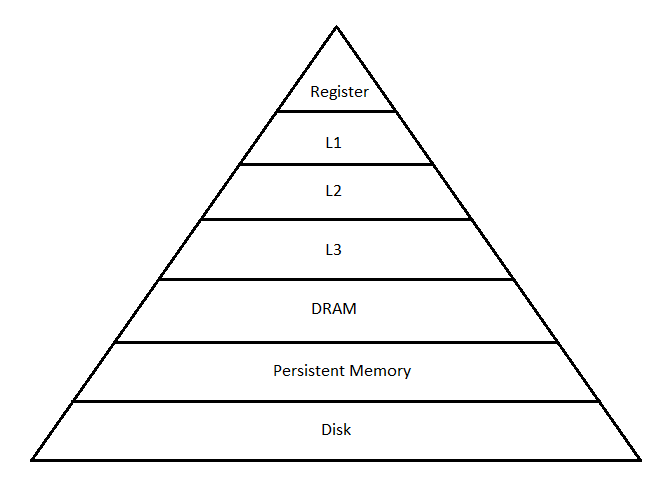
\includegraphics[scale=0.85]{Intro/Pyramid.png}
\caption{Persistent memory becomes a new level between DRAM and Disk\cite{optane}}
\label{fig:Pyramid}
\end{figure}

\subsection{Challenges}

\subsubsection{Security}
Another challenge when it comes to persistent memory is security and privacy\cite{Badam}. When an encryption key is used to unlock files, the key is stored in the memory. If it is DRAM then the key will disappear when the computer is shut down, but if it is stored in persistent memory it will persist and remain there until it is deleted. It will be very easy for someone to extract data from persistent memory if the person is able to gain access to it. The same concern also applies to personal information that is being stored in the persistent memory. When developing applications that will use persistent memory and handling sensitive information the programmer needs to remember that data he puts in persistent memory will stay there until it is deleted. It’s also worth mentioning that when the data is deleted or deallocated in the memory, the OS makes the space available to another application. The data is only deleted when its overwritten.

\subsubsection{Durability}
Another challenge for persistent memory is durability. While persistent memory behaves more like DRAM it still has a considerably shorter lifespan than DRAM\cite{Badam}. This is because persistent memory can only write data to a certain amount of time to a region before the region can no longer hold any data reliably. While the storage capacity of persistent memory has increased, so has the bit error rate increased even more. The solution to this is to either have the hardware mask all the regions with bit error from the software or have the hardware expose them to the software and let the software handle the rest. There is also the possibility of letting the hardware and software work together in order to mask regions with bit errors. This will expand the lifespan of persistent memory, but the challenge for hardware producers is to come up with new technologies that can increase the durability of the persistent memory.

\subsubsection{Persistent memory leaks}
A common problem one might have when programming in C are memory leaks. When the application is using normal DRAM, the memory consumed by the application can be freed just by restarting the application. If the application is using persistent memory on the other hand, then the memory consumed by the application will remain consumed even after the program has been restarted.\cite{Volos}\cite{Swanson} Memory leaks will persist a shutdown just like persistent memory will. The technology must ensure that the memory occupied on the persistent memory can be tracked down to the application that allocated the memory. By doing this it is possible to track down and remove memory leak for the persistent memory.

\subsection{Advantages}
\subsubsection{Cost}
One of the biggest shortcomings of DRAM is that it is expensive. When the amount of memory increases in a system the cost of DRAM scales nonlinearly.\cite{Badam} This has led to memory becoming a bottleneck in servers that runs programs where a lot of memory is needed. Persistent memory is more scalable in terms of cost then compared to DRAM. 

This will enable servers to have more storage capacity that can be read at almost the same speed as DRAM.

\subsubsection{Capacity, Larger physical memory}
The memory capacity of persistent memory represents a drastic increase in the size of memory that is available to the user. The biggest size of a DRAM memory module that can be bought today is 64 Gigabytes. Intel has announced a new persistent memory called Intel Optane DC\cite{side1}. This is a persistent memory that is compatible with a DDR4 socket and each memory module can contain 512 Gigabytes of memory. The bigger memory size will make it possible to keep more of the data the user is working on in the memory and reduce the traffic between the memory and the hard drive.

\subsubsection{Byte addressable, low latency}
Since the persistent memory is connected to a DRAM slot it is also byte-addressable. When a program accesses traditional storage it must wait for the OS to do an I/O block in order to get access which takes a long time and read/write are done in 4 kB blocks. With persistent memory the program can skip the I/O block and access the data directly, this will dramatically decrease the latency. Typical latency when using DRAM would be around 10\textsuperscript{-7}\cite{lerebok} while Intel has measured their Optane DC to have a latency of 4.1 ms\cite{optane2}. Persistent memory is 40 times slower than normal DRAM, but it is still a lot better than SSD that can have 80 ms latency.

\subsection{The rest of thesis}
In Chapter two there will be an explanation of how to program with NVDIMM. There will be an explanation of some of the different type of libraries that exist. How to set up a memory pool that will be used by the programmer and an explanation of method that will be most used by the programmer. 

In chapter three will contain several benchmarks that will show the performance of DRAM and NVDIMM when whey are working alone and when they are working simultaneously. There will also be an comparison to see if DRAM and NVDIMM are working faster or slower together when compared to DRAM working alone.

Chapter four there will be about a scenario that a programmer can encounter. That is when the data exceed the the total capacity of DRAM and the programmer is forced to split the data in two part and place the part that exceed DRAM on NVDIMM. There will be a a formula that calculate how many threads should be reallocated to work on NVDIMM.

Chapter five will also be about a different scenario. There will be a program with two part. Part one is data is calculated on DRAM by a group of threads. Part two will also have a group of threads that will first transfer the calculated data from DRAM to NVDIMM and analyze the data on NVDIMM. 

Chapter six will contain a summary and a conclusion.

\subsection{Research questions}
This thesis will try to answer the following research questions.
\begin{itemize}
\item What is the data transfer speed of NVDIMM compared to DRAM?
\item In an competitive competition how does NVDIMM and DRAM affect each other?
\item When the size of the data is higher than the capacity of the DRAM. How much data should be transferred to NVDIMM? How many threads should be allocated to work on the data on NVDIMM?
\item While DRAM is working on a task, is it possible for NVDIMM to be working on a different type of task?
\end{itemize}

% - What is the speed of NVDIMM compared to DRAM?\\
% - How does NVDIMM and DRAM interact with each other?\\
% - In an competitive competition how does NVDIMM and DRAM affect each other?
% - How many threads should the user allocate to NVDIMM when data is divided between DRAM and NVDIMM?\\
% - Something about simulation.\\

%\nocite{*}
%\nocite{*}
%\bibliographystyle{unsrt}
\printbibliography

\end{document}